% ChromDecode-At manuscript, formatted for npj Microgravity (Article).
%
% Every number in the Results is read from a CSV in ../supplementary_tables/ or
% ../data/derived/ (cited as Table Sx / Dx) or, where noted, from a plotted value in a
% figure in ../figures/. The text is converted from ../reports/manuscript_draft_v1-v8.md
% and extended with v9-v10 from ../reports/report_chromdecode_at.md (sections 17.2-17.3).
% references.bib entries were each confirmed by a live Crossref/PubMed lookup
% (see REFERENCES_REPORT.md). See BUILD.md for how to build.

\documentclass[11pt,a4paper]{article}

\usepackage[utf8]{inputenc}
\usepackage{lmodern}
\usepackage[T1]{fontenc}
\usepackage[margin=2.4cm]{geometry}
\usepackage{graphicx}
\usepackage{booktabs}
\usepackage{amsmath}
\usepackage[hidelinks]{hyperref}
\usepackage[numbers,sort&compress]{natbib}
\usepackage{authblk}
\usepackage{caption}
\usepackage{subcaption}
\usepackage{microtype}
\usepackage{lineno}

\captionsetup{font=small,labelfont=bf}
\graphicspath{{../figures/}}
\linenumbers

\newcommand{\ChromDecode}{ChromDecode-At}
\newcommand{\Sx}[1]{Table~S#1}

\title{\bfseries Expression-to-chromatin decoding of the \textit{Arabidopsis}
spaceflight transcriptome reveals a robust Polycomb-state bias in repressed genes
that is not a SOG1 damage response}

\author[1]{Richard J. Barker\thanks{ORCID 0000-0001-5681-9857. Correspondence: richard@cosecloud.com}}
\affil[1]{Center of Space Exploration (CoSE)}
\date{}

\begin{document}
\maketitle

\begin{abstract}
\noindent
Spaceflight reprograms the plant transcriptome, but how these transcriptional changes
relate to chromatin organisation is unexplored, largely because no spaceflight
epigenomic assay exists for \textit{Arabidopsis}. We built \ChromDecode{}, a
reproducible pipeline that decodes any \textit{Arabidopsis} expression dataset into
the chromatin-state language of the Plant Chromatin State Database (PCSD; 36 ChromHMM
states) and AraENCODE (12 states), and applied it to every \textit{Arabidopsis} RNA-seq
dataset in NASA's Open Science Data Repository (OSDR; 33 accessions). Genes
down-regulated by spaceflight are strongly concentrated in Polycomb-repressed
chromatin: in OSD-37 seedlings, the AraENCODE Repression state has an odds ratio of
8.0 (FDR $3\times10^{-105}$) and PCSD state S15 (H3K27me3 + accessible DNA) one of 18.0. The
direction replicates, with a smaller effect, in an independent ISS centrifuge dataset (OSD-314) once its
microgravity and Mars-gravity arms are analysed separately. After sample metadata was recovered from NCBI BioSample
for datasets with undocumented designs, the signal also replicates in ISS-grown roots in two ecotypes (odds
3.1--3.7, FDR $<10^{-6}$; Col-0 in OSD-193 and OSD-218, and WS in OSD-218). A pre-submission audit
re-derived every contrast from the OSDR study records and corrected three sample-coding errors (Fig.~\ref{fig:qc}). The repressed class is a
coherent peroxidase and oxidant-detoxification module (11 GO terms significant even
against a state-matched Polycomb control). Its promoters are enriched for AT-hook (AHL)
and ZHD-family motifs, an architecture that tracks the Polycomb state itself rather
than the flight response. A reanalysis of the only \textit{Arabidopsis} ChIP-seq in
OSDR (SOG1-3xFLAG after bleomycin-induced DNA damage) finds no SOG1 binding at
redox-module or Polycomb-down promoters, which excludes the canonical SOG1-dependent
damage-repression pathway. Whole-genome bisulfite data (OSD-217) show no significant
flight-induced methylation change at the module. A power analysis indicates that
$\sim$9--12 replicates per group are needed for a stable root-level enrichment test,
and a stratified analysis of OSD-120 shows that its 12-sample design cannot resolve a
flight $\times$ light interaction. The Polycomb-state bias of the spaceflight
repression response is robust across tissues and campaigns, is not a SOG1-style
damage response, and its upstream regulator remains unidentified. It is a concrete,
testable target for spaceflight epigenomics.
\end{abstract}

\noindent\textbf{Keywords:} \textit{Arabidopsis thaliana}; spaceflight; chromatin
states; Polycomb; H3K27me3; PCSD; AraENCODE; NASA OSDR; RNA-seq; SOG1

% =====================================================================
\section{Introduction}

Plants are central to bioregenerative life support for space exploration, and their
transcriptomes respond extensively to spaceflight
\citep{gebre2025osdr,berrios2021genelab,paul2017genetic}. Chromatin state, the combinatorial pattern of histone marks,
DNA methylation and accessibility, constrains which genes a cell can express. Polycomb
repression (H3K27me3) is a canonical mechanism of stable, heritable gene silencing in
plants. Whether spaceflight transcriptional repression targets genes in a
chromatin-state-dependent manner has never been asked, because no spaceflight
chromatin assay exists for any plant. We verified that OSDR contains no spaceflight
H3K27me3 ChIP-seq; the only \textit{Arabidopsis} ChIP-seq it holds is a ground-based
DNA-damage experiment (OSD-496).

\ChromDecode{} sidesteps this gap. Given an expression dataset, it maps every gene to
its (ground-state) chromatin context using the PCSD 36-state ChromHMM model
\citep{liu2018pcsd,ernst2012chromhmm} and AraENCODE 12-state annotations
\citep{wang2023araencode}. It then tests whether differentially expressed genes are concentrated
in particular chromatin classes. Here we present the full analysis programme:
decoder construction and validation, a learned expression-to-state model (negative),
an OSDR-wide sweep at three state resolutions, robustness diagnostics, functional
characterisation of the repressed module, methylation tests, a SOG1 ChIP-seq mechanism
test, a tissue-matched root replication with metadata forensics, a power analysis, and
a flight $\times$ light interaction bound.

% =====================================================================
\section{Results}

\subsection{A hybrid decoder validates on OSD-37}

\ChromDecode{} harmonises AGI identifiers and computes differential expression
(linear models with ecotype covariates, BH-FDR \citep{benjamini1995fdr}). It maps genes to
chromatin states via TSS-anchored coordinates (gene body + 2\,kb upstream; 100\% PCSD
and AraENCODE coverage; 37.7\% PlantCADB ACR overlap \citep{ding2023plantcadb}), and tests
state enrichment of up- and down-regulated genes against the expressed genome with
Fisher's exact test (Table~D1).

The first validation run used GeneLab VST counts for OSD-37 (28,067 genes $\times$ 56
samples; four ecotypes; 117 up / 53 down at padj $<0.05$, $|\log_2\mathrm{FC}|>1$;
\Sx{1}). Up-regulated genes were enriched for accessible-promoter chromatin (odds 3.22,
FDR $3.0\times10^{-7}$) and depleted from heterochromatin/TE (0.28) and Polycomb states
(0.32; \Sx{2}). Down-regulated genes were strongly enriched for Polycomb-repressed
chromatin (odds 11.46, FDR $1.4\times10^{-14}$) and depleted from accessible promoters
(0.14; \Sx{3}; Fig.~\ref{fig:decoder}). The two independent state annotations agreed,
and locus controls behaved correctly: \textit{FLC} fell in a repression state, while
\textit{ACT2} and \textit{PHYB} were active (Fig.~S1).

\subsection{A learned expression-to-state model fails honestly}

An elastic-net multinomial model predicting state group from eight
expression-distribution features reached a CV accuracy of 0.513 against a majority
baseline of 0.588 (\Sx{4}). Version 2 retrained it on tissue-matched pairs: AraENCODE seedling
expression, 28,727 genes and 11 features including tissue-specificity statistics.
It used nested CV and genomic-block CV (100-kb bins) and reached accuracy 0.533--0.554 against
a baseline of 0.549. Transfer to leaf, root and OSD-37 spaceflight data was $\le0.548$
in every case (\Sx{7}, \Sx{9}). Expression distributions do not predict chromatin state.
The block CV shows the negative is not a CV artefact, and it motivates the
deterministic coordinate-based backbone that carries every later analysis.

\subsection{An OSDR-wide sweep: the signal replicates}

The backbone ran on every \textit{Arabidopsis} RNA-seq dataset in OSDR (33
accessions), with contrasts auto-detected from metadata and sample-name conventions
(\Sx{10}). It produced full DE + enrichment for 5 datasets and expression-only decoding
for 18; 10 had no processed counts. DE was computed on log$_2$-transformed counts with
ecotype covariates. An earlier raw-scale version inflated DE roughly fivefold and was
corrected. Under the corrected model, OSD-37 \citep{choi2019variation} yielded 529 up / 526 down genes
(\Sx{52}). Re-running the sweep for all five DE datasets reproduced every count and every
12- and 36-state odds ratio exactly (\Sx{50}). It also regenerated the corrected 5-group
enrichment (\Sx{51}): OSD-37 down-regulated genes are enriched for Polycomb\_repressed (odds 7.01, FDR
$1.7\times10^{-92}$) and depleted from Heterochromatin\_TE (0.07) and Accessible\_promoter (0.38).

At AraENCODE 12-state resolution (\Sx{11}; Fig.~\ref{fig:sweep}), down-regulated genes
were enriched for the Repression (Polycomb) state in OSD-37 (odds 8.0, FDR
$3\times10^{-105}$). OSD-314 \citep{villacampa2021mars} is treated separately below because the sweep mis-coded its
design. OSD-37 up-regulated genes
were enriched for Active (1.57) and Transcription2 (5.4) and almost absent from
Heterochromatin (0.03). At PCSD 36-state resolution (\Sx{12}), OSD-37 down-regulated
genes converged on the H3K27me3/accessible-promoter block. Odds were 18.0 for S15 (H3K27me3 + accessible DNA),
6.4 for S16, 3.9 for S14 and 3.3 for S13 (all FDR $<0.001$).
Of the 526 OSD-37 down-regulated genes, 265 sit in Polycomb states S11--S15.
Constitutive heterochromatin (S29--S36) was depleted in both directions across datasets.
Spaceflight-repressed genes are therefore a coherent class of promoter-accessible,
Polycomb-marked euchromatic genes. One derived claim from the uncorrected DE (OSD-314 down genes in Active chromatin) is
retracted.

\subsection{OSD-314: the direction replicates, the magnitude does not}

OSD-314 is a three-arm ISS centrifuge experiment: 0\,g ($n=5$), 1\,g ($n=6$) and Mars 0.3\,g ($n=6$),
crossed with red light or darkness (Table~S53). The sweep's sample-name parser recognised the 0G and 1G tokens but not
``03g''. The contrast-coding step then treated the six unparsed Mars-gravity samples as treatment, so the
published contrast was 0\,g + 0.3\,g pooled (11) against 1\,g (6), with no light term. Coding gravity and light
explicitly (\Sx{54}) gives far more DEGs: 1,457 up / 1,921 down for 0\,g vs 1\,g, and 1,105 / 1,238 for
0.3\,g vs 1\,g, both with light as a covariate (\Sx{55}--\Sx{56}).
The Polycomb bias of down-regulated genes keeps its direction at a much smaller magnitude. AraENCODE
Repression odds are 1.38 (FDR $2.7\times10^{-6}$) for 0\,g and 2.04 (FDR $2.6\times10^{-21}$) for 0.3\,g. The 5-group
Polycomb odds are 1.23 and 1.76 (Fig.~\ref{fig:qc}a). All 0\,g sample identifiers share a different prefix from the
1\,g and 0.3\,g samples, which suggests a separate processing batch. We could not confirm this from the study record,
so the 0\,g contrast may be batch-confounded.

\paragraph{Up-regulated genes.} In the published (pooled) contrast, OSD-314's 47 up-regulated genes were
strongly enriched for Polycomb CDS states: S11 (odds 22.4), S12 (4.2) and S13 (5.7) (\Sx{12}). Under correct coding,
up-regulated genes remain enriched for Polycomb chromatin (5-group odds 2.59 and 2.76, FDR $<10^{-40}$) and for S11
(odds 2.05, FDR $4.5\times10^{-5}$; and 1.95, FDR $6.8\times10^{-4}$). The ``escape from Polycomb repression'' reading
therefore survives in direction, but at about a tenth of the published S11 effect (Fig.~\ref{fig:qc}b).
The five diagnostics below were run on the published 47-gene set (Fig.~\ref{fig:osd314}). They show that the set is not a
small-sample artefact, but they cannot correct its contrast.
(i) Null calibration with 10,000 random 47-gene draws gives S11 an empirical $p<10^{-4}$, S12 0.0013
and S13 0.0036 (\Sx{13}). (ii) Downsampling OSD-37's up-regulated genes to $n=47$ never
reached the observed S11 or S12 odds (\Sx{14}). (iii) In a threshold grid, S11 odds rise
with DE stringency, from 1.3 ($n=456$) to 2.3 ($n=241$) to 3.8 ($n=88$) at padj $<0.01$, and reach 6.7 ($n=189$)
at padj $<0.05$, $|\log_2\mathrm{FC}|>2$ (\Sx{15}). (iv) Threshold-free GSEA on 1,944 Polycomb genes gives a
permutation $p<0.001$ (\Sx{16}). (v) Of the up-regulated genes, 29 sit in Polycomb states and
include adjacent pairs, which suggests tandemly duplicated clusters (\Sx{17}). An S15
enrichment previously reported for these genes came from the uncorrected DE
(empirical $p=0.51$) and is retracted. Under both corrected contrasts, genes held in H3K27me3-marked chromatin
are still disproportionately \emph{released} in altered gravity, but modestly.

\subsection{The repressed class is a redox/peroxidase module in AHL/ZHD promoter architecture}

We compared three gene sets: the target (Polycomb-down, $n=265$), control 1 (non-Polycomb-down,
$n=241$) and control 2 (state-matched Polycomb non-DE, $n=3{,}303$).

\paragraph{GO.} Against the genome, 18 terms were significant (TAIR GAF, hypergeometric,
BH-FDR \citep{go2023knowledgebase}; \Sx{19}), dominated by oxidative stress. They include peroxidase activity
(11.1$\times$), heme binding (7.2$\times$), hydrogen peroxide catabolic process
(13.6$\times$) and cellular oxidant detoxification (8.8$\times$). Eleven terms
remain significant against the state-matched Polycomb control, so the flight-repressed
subset is functionally a redox module, not a random Polycomb slice
(Fig.~\ref{fig:module}).

\paragraph{Motifs.} We scanned 897 JASPAR 2024 plant motifs \citep{rauluseviciute2024jaspar} over strand-aware 2\,kb promoters
with per-motif $p<10^{-4}$ thresholds (\Sx{18}). Against the genome, 268 motifs were significant.
They include ZHD1 (2.9$\times$), the AT-hook family AHL12/13/25 (up to 5.7$\times$) and NTL9.
No motif survives BH-FDR against the state-matched control (best nominal: NTL9, odds 2.1, padj
0.084), so the motif layer tracks the Polycomb state, not the response. Promoter GC
content is similar (target 0.310 vs control 2 0.320; \Sx{20}), which excludes GC artefacts.
In OSD-314, 8 of 10 top GO terms replicate directionally (folds 7--27$\times$), a
result limited by power to 18 Polycomb-down genes (\Sx{21}). These genes come from the pooled contrast
described above, so this replication should be repeated on the corrected 0.3\,g contrast.

\subsection{No flight-induced methylation change at the module}

With no spaceflight H3K27me3 data, we tested the slow-turning epigenetic layer using
OSD-217 \citep{zhou2019epigenomics}: Ws ecotype, root and leaf WGBS, flight vs ground. These
data were processed by the authors against the ecotype-matched Ws assembly
\citep{xi2009bsmap,sun2014moabs}. Gene-body tests found no significant change for the 23-gene redox module (minimum padj 0.07;
root CHG nominal $p=0.012$; \Sx{22}). Promoter-window tests (2\,kb, 100-bp bins, 21,424 genes) also found nothing that
survives BH-FDR (minimum padj 0.099; \Sx{23}--\Sx{24}). The module shows directionally
consistent nominal CHG gains in both tissues ($p\approx0.011$). Baseline promoter CG
methylation of the Ws-defined Polycomb-down module is elevated in root (median 0.52 vs
0.02, $p=0.043$, $n=6$; not BH-significant). Flight log$_2$FC correlates only weakly between OSD-217
(Ws root) and OSD-37 (Col-0 seedlings): $r=-0.17$ over 63 genes (\Sx{25}). This reflects
ecotype, tissue and campaign confounding, and motivates the tissue-matched replication below.

\subsection{SOG1 does not bind the module: excluding the damage-response pathway}

SOG1 is the plant NAC-family master regulator of the DNA-damage response
\citep{yoshiyama2009sog1}. If spaceflight repression of the redox module were a SOG1-style damage
response, SOG1 should occupy the module's promoters. We reanalysed OSD-496 \citep{bourbousse2018sog1}:
SOG1-3xFLAG seedlings treated with bleomycin, six single-end libraries of 13.7--23.4\,M reads. We aligned the reads to TAIR10
with HISAT2 \citep{kim2019hisat2} (\texttt{--no-spliced-alignment}) and called MACS2 \citep{zhang2008macs}
narrow peaks ($q<0.01$, IP vs matched-timepoint input). This gave 56 peaks at 20\,min and 100 at 1\,h.
SOG1-IP vs wild-type-IP gave 160/180 peaks. Of the 1-h peaks, 67/100 overlap a 2\,kb promoter, and the median
peak-to-TSS distance is 194\,bp.

The result is a clean negative (\Sx{26}; Fig.~\ref{fig:sog1}). Across the peak union,
no SOG1 peak falls in a redox-module promoter (0/23) or a Polycomb-down promoter (0/265)
at either timepoint (all Fisher padj = 1.0). Three of 3,303 background promoters are
bound. The spaceflight repression of the module is therefore not a recapitulation
of SOG1's direct damage targets.

\subsection{Tissue-matched root replication, with metadata forensics}

We enumerated all 62 \textit{Arabidopsis} OSDR studies (33 with RNA-seq, 10 mentioning root
tissue) and resolved the field by QC (\Sx{27}). Each candidate's platform and genotypes were then re-read
from its OSDR study record and BioSample titles during the pre-submission audit. ISS root datasets:
OSD-120 (CARA root tips \citep{paul2017genetic}), and OSD-193 \citep{califar2020root} and OSD-218, both from the
APEX-03-2 payload. OSD-193 and OSD-218 ship counts keyed by GSM/SAMN accessions with empty OSDR factor values,
so every sample ID was resolved to its condition via NCBI BioSample (e.g.\ ``Spaceflight, 8 days old, Col-0
Rep4''; Tables~D4--D7). OSD-193 is Col-0 and \textit{sku6}; OSD-218 is Col-0 and WS (16 samples each).
Suborbital datasets: OSD-624, Col-0 on Virgin Galactic Unity~22 \citep{ferl2023virgin}; and OSD-406, Col-0, WS and
\textit{sku5} on Virgin Galactic VP-03 and Blue Origin NS-12 \citep{califar2021suborbital}. OSD-281 was excluded on recovery
because it holds 16 \textit{sku5}-mutant and 16 Ws samples and no Col-0. Documented exclusions are OSD-217 (Ws),
OSD-219/427 (no counts), OSD-411/480 (EMCS partial gravity) and OSD-208 (no flight factor).

\paragraph{ISS roots.} With age as a covariate, OSD-193 Col-0 WT (8 v 8) gave 97 up / 181 down, Polycomb odds 3.06,
padj $2.2\times10^{-10}$ (\Sx{29}, \Sx{31}--\Sx{32}). The v8 run of OSD-218 entered all 32 samples as ``Col-0''
because the BioSample parser did not recognise ``WS''. Re-run by genotype (\Sx{48}), Col-0 alone (8 v 8) gives
96 up / 182 down, odds 3.12, padj $7.6\times10^{-11}$ (\Sx{49}), and WS alone (8 v 8) gives 81 / 82, odds 3.74,
padj $6.5\times10^{-7}$. The pooled run with genotype as a covariate gives odds 3.06. The v8 pooled estimate
(odds 3.14, padj $4.7\times10^{-7}$; \Sx{33}--\Sx{34}) is therefore numerically unchanged, but it is now
attributed correctly: the root-level Polycomb bias replicates in \emph{two ecotypes}. OSD-120 restricted to Col-0 WT
collapses to 2 down genes after light/day covariate control (\Sx{38}--\Sx{39}); its power is examined below.

\paragraph{Suborbital roots.} OSD-624 (minutes of microgravity on a suborbital flight) is null: 36 down genes,
odds 0.76, padj 0.81 (\Sx{35}--\Sx{37}). The v8 analysis treated OSD-624 as an orbital root dataset and read
its null as a campaign difference. The study record shows it is suborbital, so the null no longer weighs against
the ISS replications. The v8 run of OSD-406 pooled three genotypes and two rockets with no covariates and found
1 down gene (\Sx{40}--\Sx{41}). With genotype and rocket as covariates it gives 23 up / 38 down, Polycomb odds
3.17, padj 0.0074 (\Sx{48}). Genotype and rocket are partly confounded in that design (\textit{sku5} flew only on
Blue Origin, Col-0 only on Virgin Galactic), so we treat this as a discovery-level observation. The Col-0 subset
alone (3 v 3) has no DEGs.

In summary, the Polycomb enrichment of flight-repressed genes replicates in every adequately powered ISS root
contrast (OSD-193 Col-0; OSD-218 Col-0 and WS) at roughly half the seedling effect size. The corrected 5-group
Polycomb odds for OSD-37 is 7.01 (\Sx{51}). OSD-193 and OSD-218 share the APEX-03-2 payload, so they are not fully
independent replications.

\subsection{Power: replicates needed for a stable root-level enrichment test}

How many replicates would a root study need? Effect sizes were anchored to this project's
own observations (odds 3.1 at root level, 7.0 at seedling level) with a background Polycomb fraction
of 0.141 (4,812 of 34,054 genes), $\alpha=0.05$ and 80\% power. Simulating the enrichment test alone shows
that $\sim$40 down-regulated DEGs are needed at root-level odds, or $\sim$15 at seedling-level
odds (Fig.~\ref{fig:roots}b; \Sx{42}). Running the full pipeline on $k$ replicates per group
subsampled from OSD-218 (20 draws each; \Sx{43}), power is 0--15\% at $k=2$--6, 50\% at $k=8$, and 100\% at
$k=12$--16 in a clean design. At $k=16$ the draws reproduce the full result exactly (117 down genes),
which validates the pipeline. Interpolating gives $\sim$9--10 replicates per group in a clean design and
$\sim$11--12 with OSD-120's light $\times$ day covariate burden. OSD-120's Col-0 WT contrast
(6 v 6) sits at $\sim$10--15\% power. The subsampling pool mixes the Col-0 and WS samples of OSD-218 without a
genotype term, which adds draw-to-draw composition noise, so these replicate numbers are conservative design estimates.

\subsection{Bounding the flight $\times$ light interaction in OSD-120}

The additive model's collapse could hide a real flight $\times$ light interaction absorbed into the
light term. The Col-0 WT design is a balanced 2$\times$2 factorial (FLT/GC $\times$
Alight/dark, 3 replicates per cell, all Day 13), so the interaction is directly estimable
(\Sx{44}--\Sx{47}; Fig.~\ref{fig:roots}c). Within Alight there were 1 up / 0 down genes; within dark, 2 up / 1 down,
the latter not in a Polycomb state. The Polycomb-down module (37 genes taken from the pooled Col-0 + WS OSD-218 run) trends down within Alight
(median log$_2$FC $-0.31$) but up within dark ($+0.16$). In the full 12-sample model
(expression $\sim$ condition + light + condition:light), only 4 genes genome-wide show
a significant interaction (padj $<0.05$, $|\log_2\mathrm{FC}|>1$), and the median $|$interaction$|$ is 0.50.
Neither the redox module (23 genes; median $|$interaction$|$ 1.26) nor the Polycomb-down
module (37 genes; median 1.18) contains a significant interaction. The additive null
is not explained by a large masked interaction. But at 3 v 3 per stratum this is a bound on
detectable interaction, not evidence of absence: OSD-120's design cannot resolve the
interaction on the Polycomb module.

% ------------------------------------------------------------- figures
\begin{figure}[p]
\centering
\begin{subfigure}{0.49\textwidth}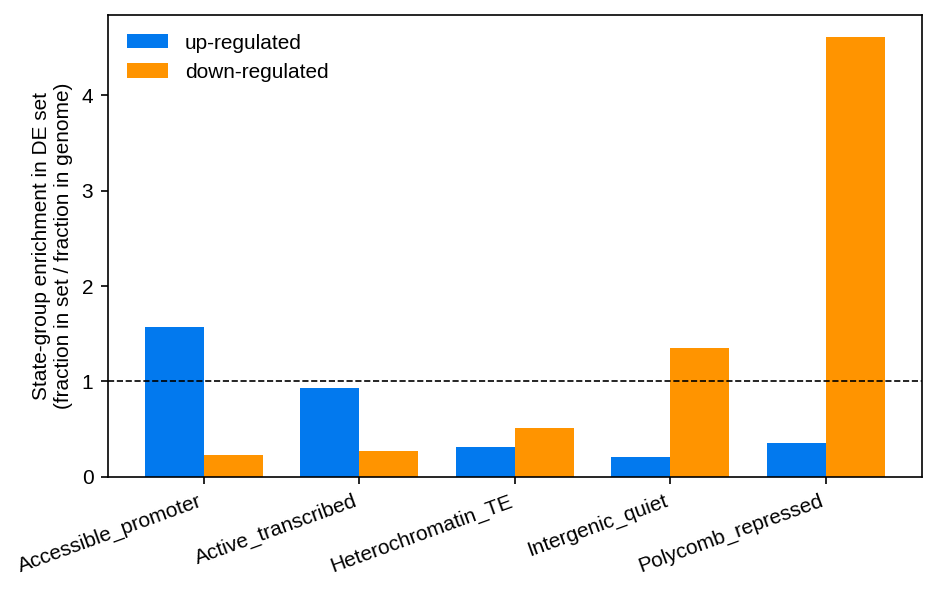
\includegraphics[width=\linewidth]{fig1_state_distribution.png}\caption{}\end{subfigure}
\begin{subfigure}{0.49\textwidth}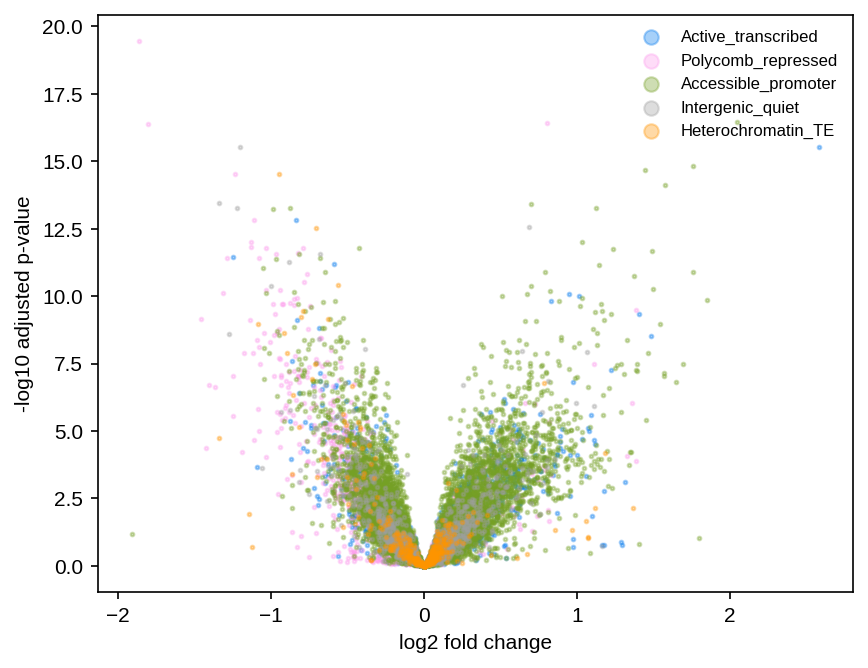
\includegraphics[width=\linewidth]{fig3_volcano_by_state.png}\caption{}\end{subfigure}\\[4pt]
\begin{subfigure}{0.49\textwidth}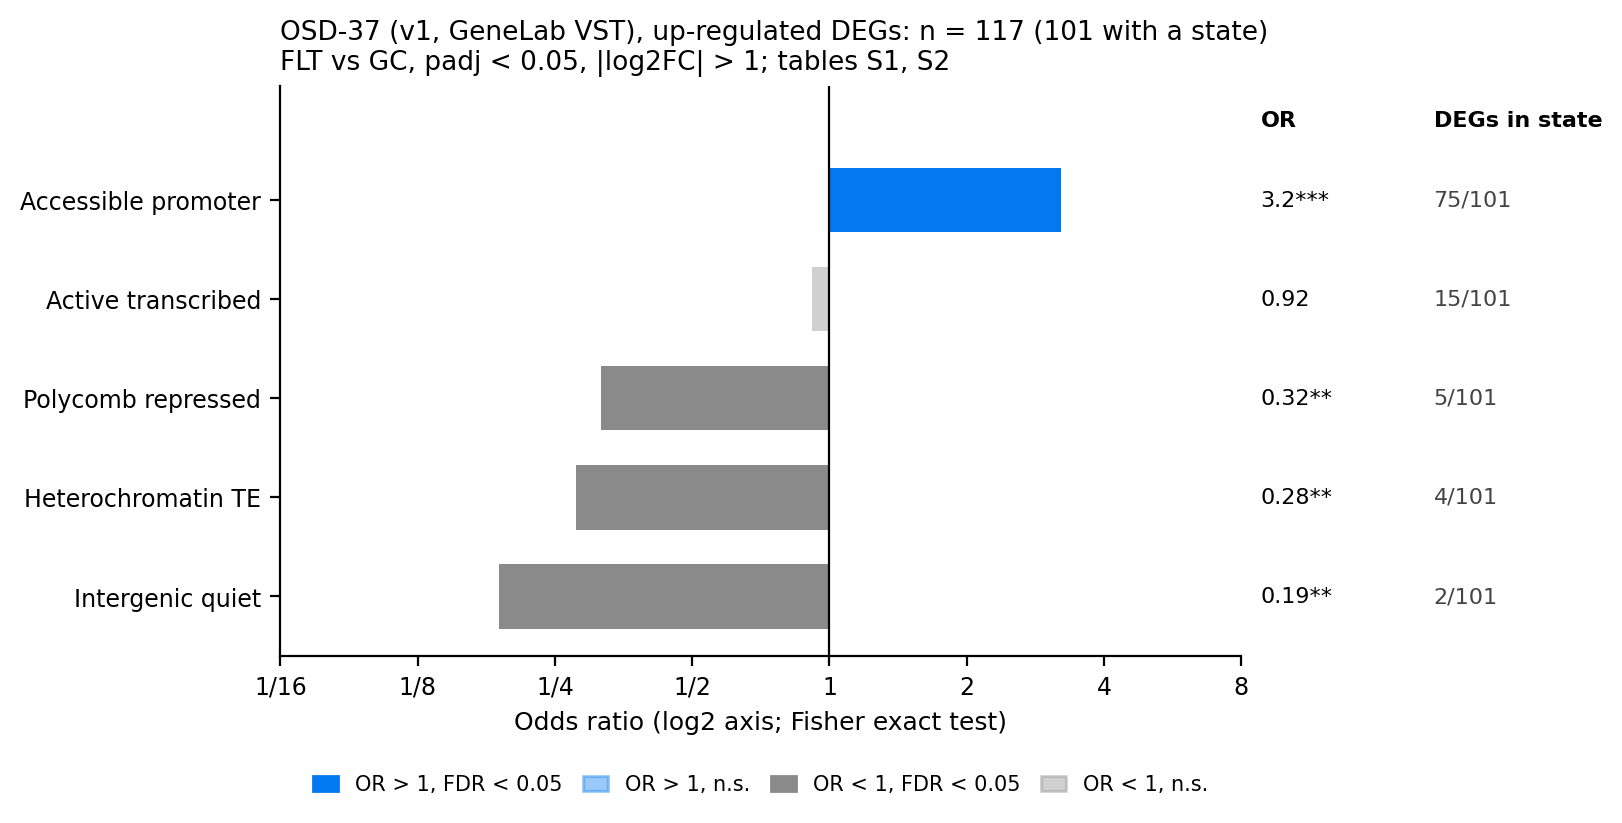
\includegraphics[width=\linewidth]{fig2_enrichment_up.png}\caption{}\end{subfigure}
\begin{subfigure}{0.49\textwidth}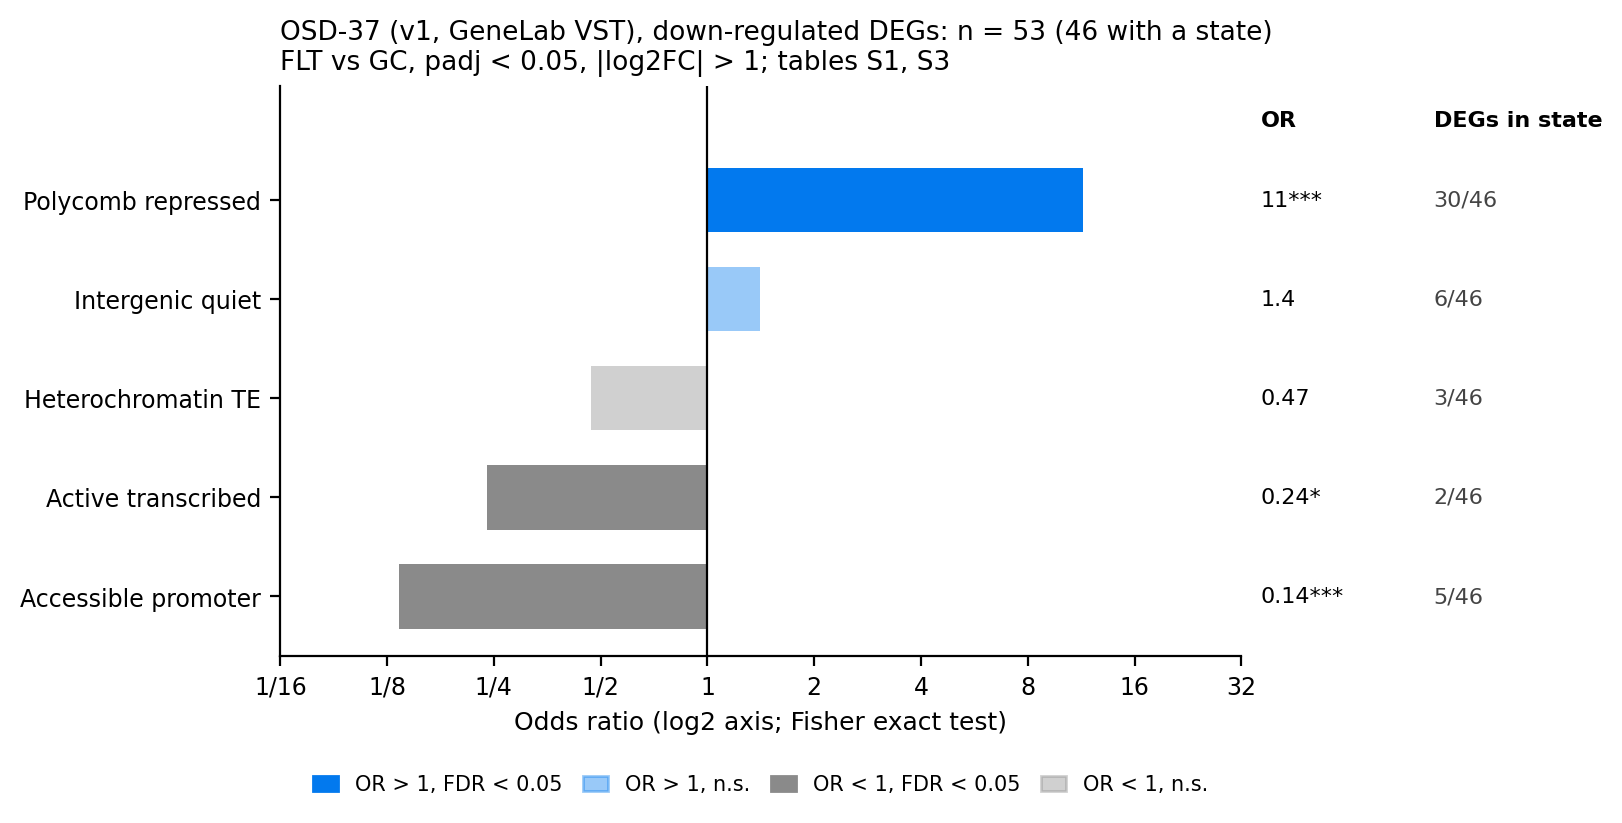
\includegraphics[width=\linewidth]{fig2_enrichment_down.png}\caption{}\end{subfigure}
\caption{\textbf{The decoder on OSD-37 (v1).} (a) Chromatin-state distribution of genes.
(b) Volcano plot coloured by chromatin-state group. (c, d) State-group enrichment of
up- and down-regulated genes (Tables~S2--S3).}
\label{fig:decoder}
\end{figure}

\begin{figure}[p]
\centering
\begin{subfigure}{0.8\textwidth}\centering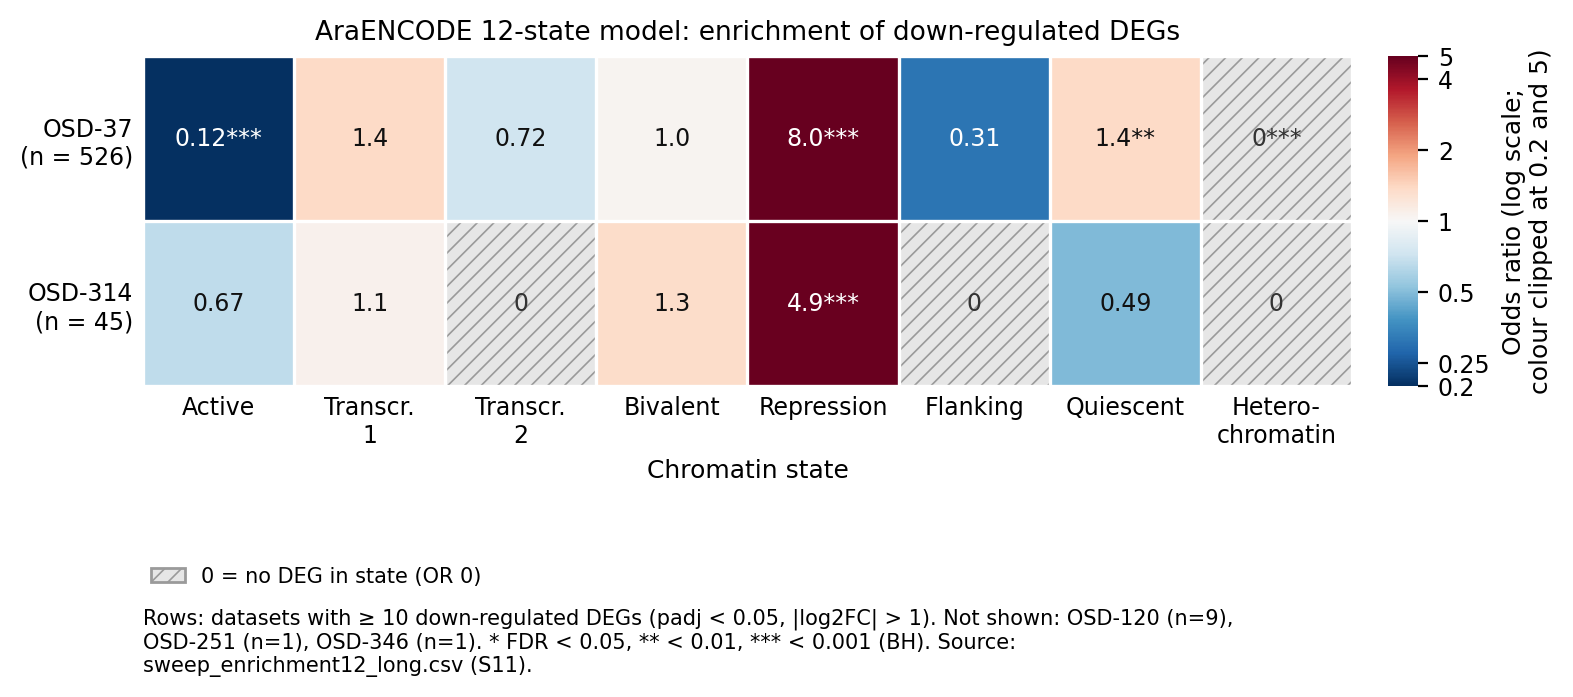
\includegraphics[width=\linewidth]{fig14_sweep_heatmap_12state_down.png}\caption{}\end{subfigure}\\[2pt]
\begin{subfigure}{\textwidth}\centering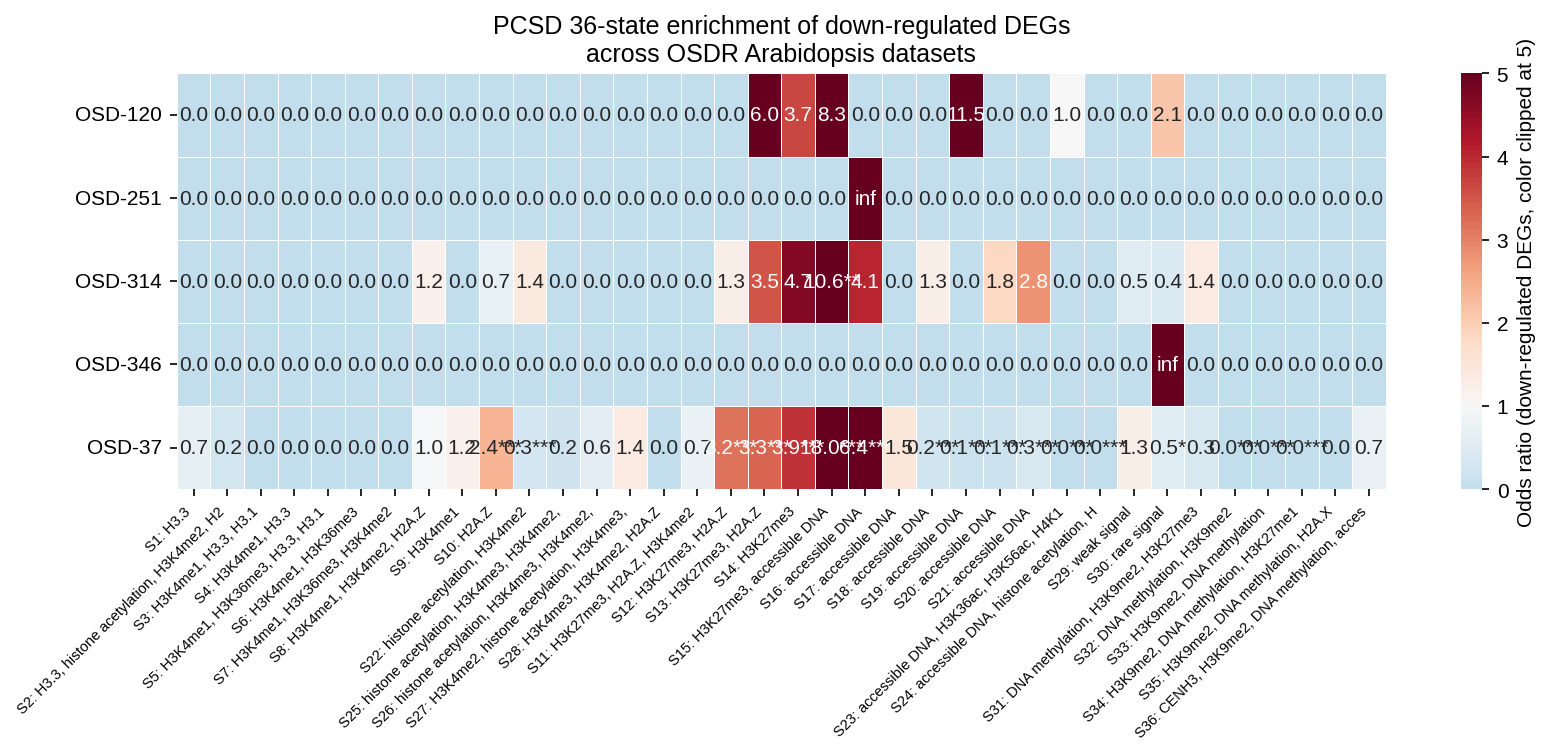
\includegraphics[height=0.56\textheight,keepaspectratio]{fig16_sweep_heatmap_36state_down.png}\caption{}\end{subfigure}
\caption{\textbf{OSDR-wide sweep: down-regulated genes concentrate in Polycomb states.}
(a) AraENCODE 12-state enrichment of down-regulated DEGs across datasets with DE
(\Sx{11}). (b) PCSD 36-state enrichment (\Sx{12}); colour is clipped at odds 0.2 and 5. Only datasets with $\ge$10 DEGs are shown, and the OSD-314
column uses the published pooled contrast (Fig.~\ref{fig:qc}).
Up-regulated counterparts are Figs.~S7--S8.}
\label{fig:sweep}
\end{figure}

\begin{figure}[p]
\centering
\begin{subfigure}{0.49\textwidth}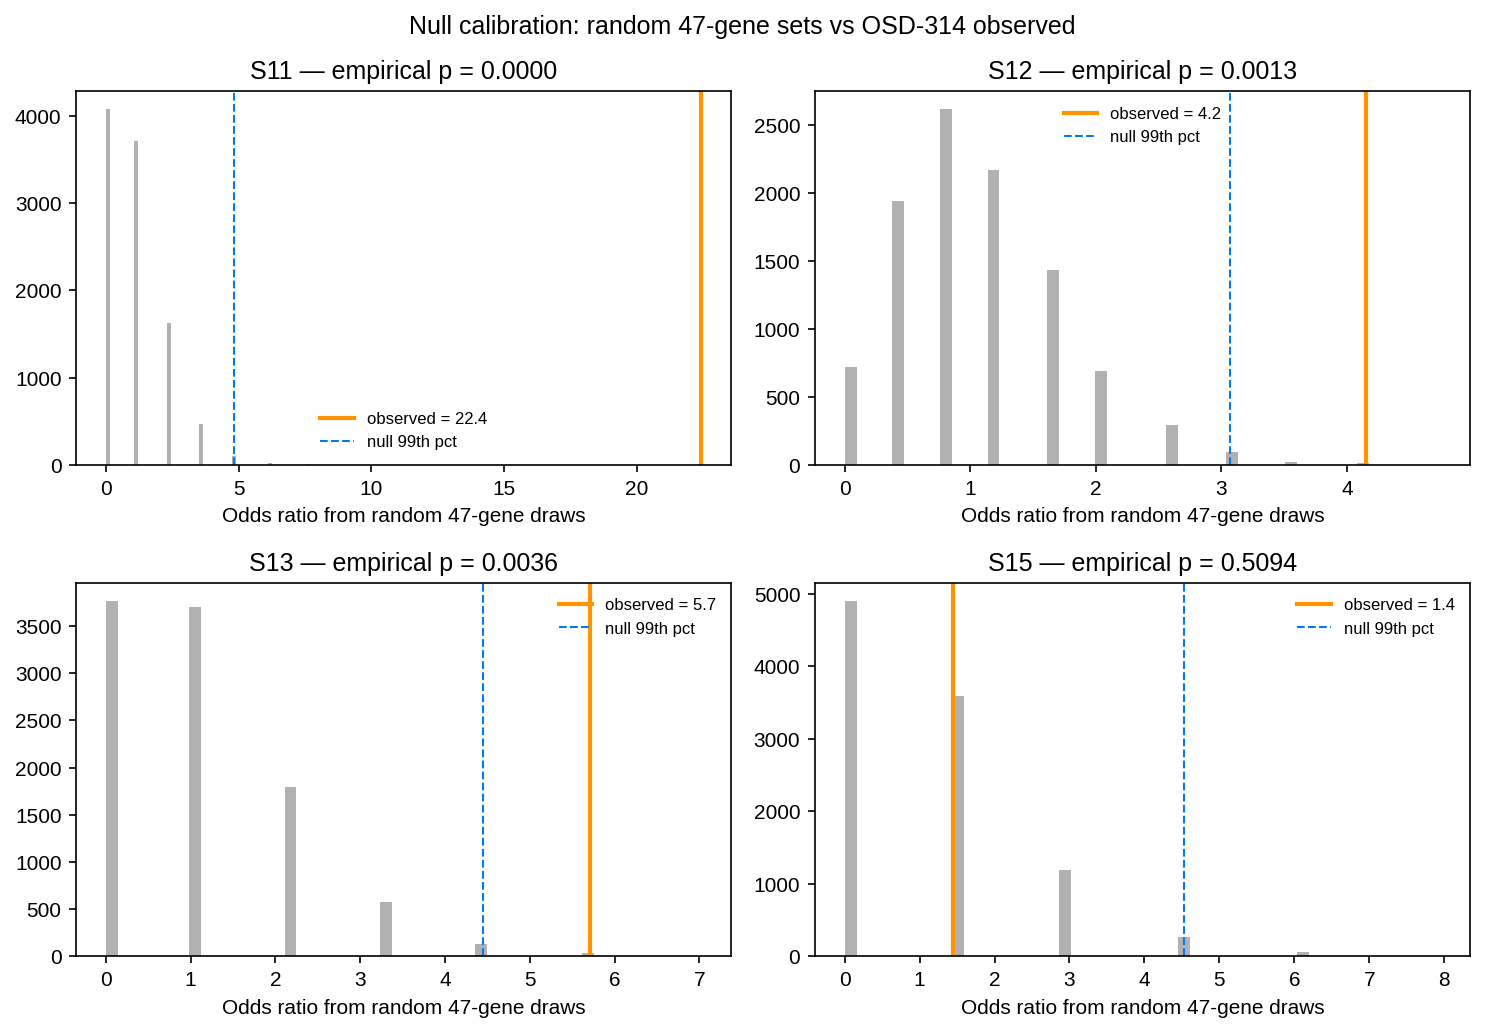
\includegraphics[width=\linewidth]{fig17_null_calibration.png}\caption{}\end{subfigure}
\begin{subfigure}{0.49\textwidth}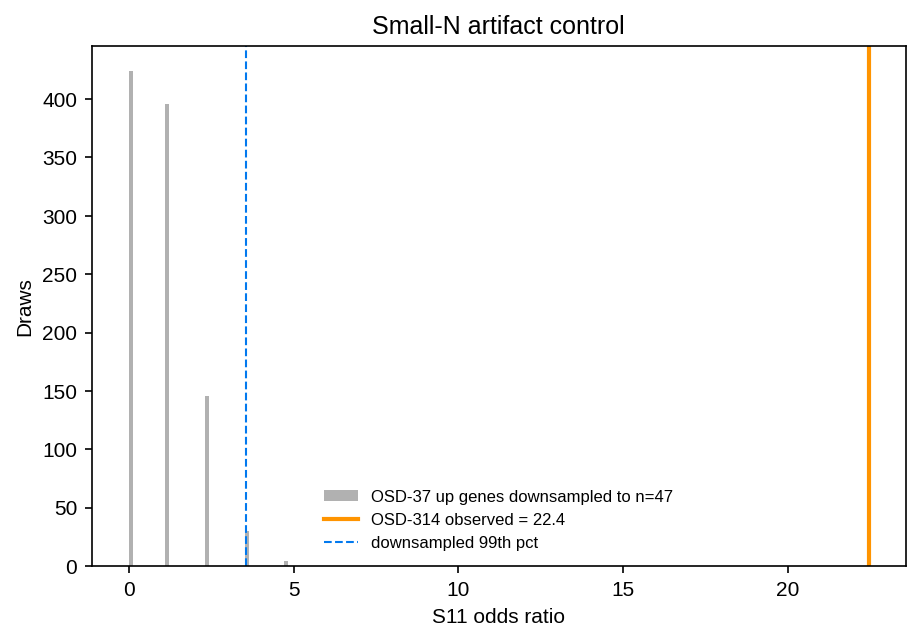
\includegraphics[width=\linewidth]{fig18_downsampling_control.png}\caption{}\end{subfigure}\\[4pt]
\begin{subfigure}{0.49\textwidth}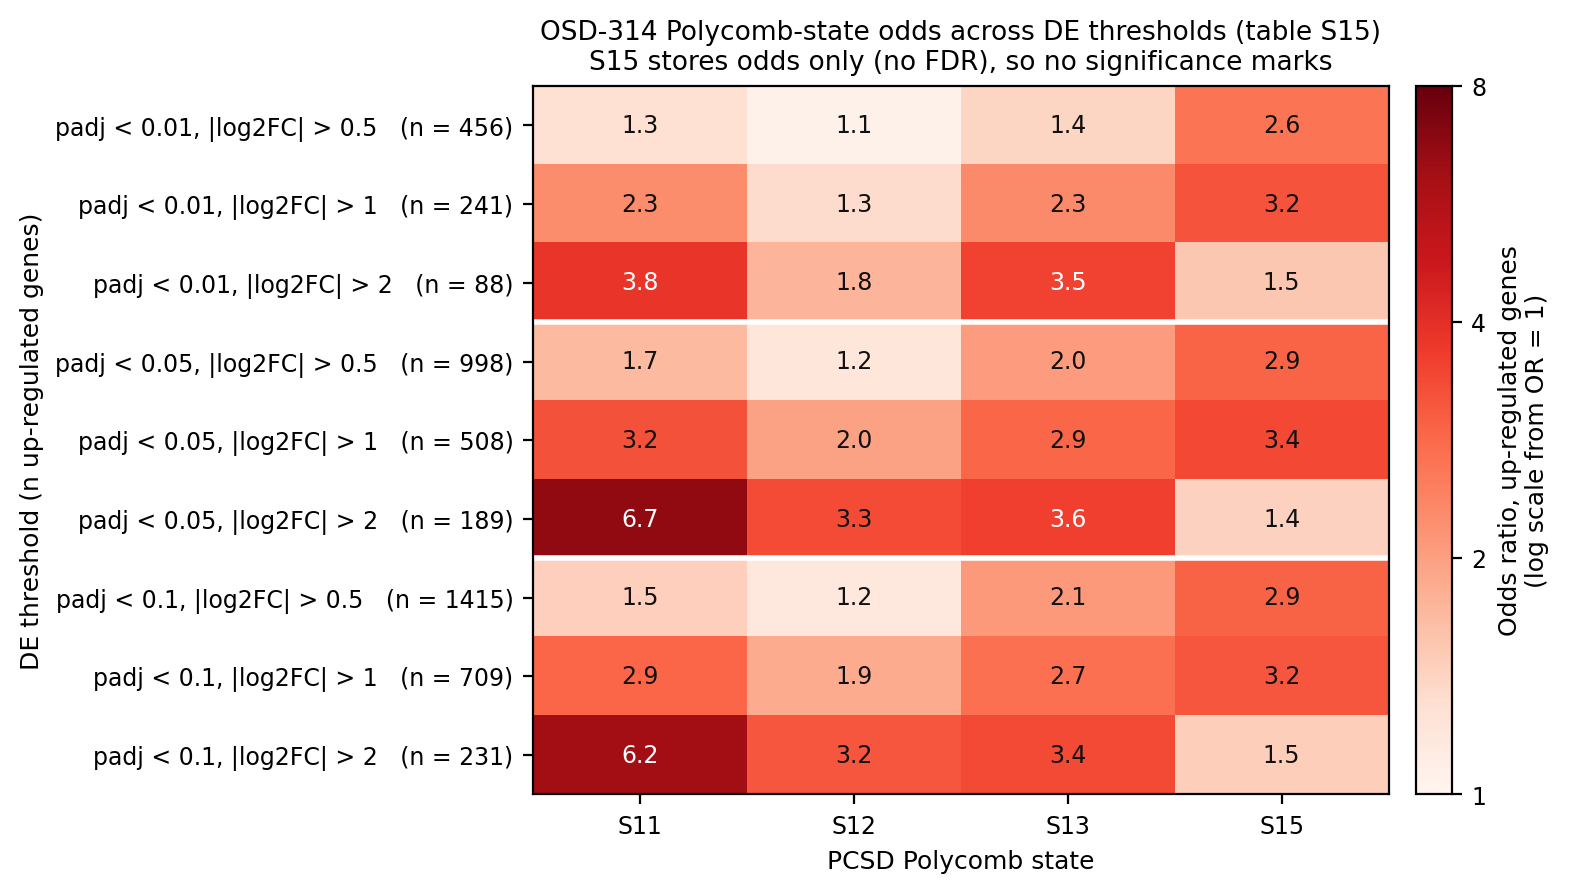
\includegraphics[width=\linewidth]{fig19_threshold_grid.png}\caption{}\end{subfigure}
\begin{subfigure}{0.49\textwidth}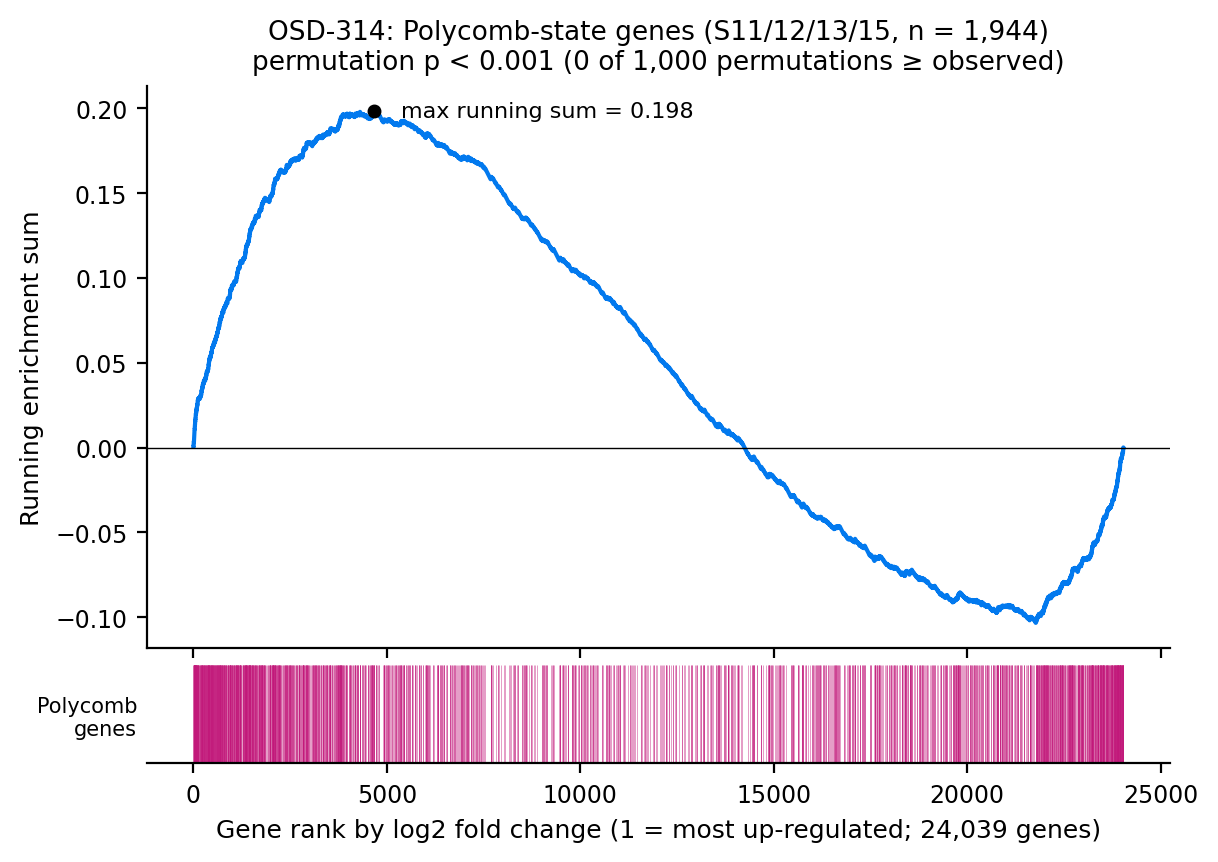
\includegraphics[width=\linewidth]{fig20_running_enrichment.png}\caption{}\end{subfigure}
\caption{\textbf{Robustness diagnostics for the published OSD-314 up-regulated gene set.} All panels use the
published contrast, which pooled the 0\,g and 0.3\,g arms (see Fig.~\ref{fig:qc}b for corrected S11 odds).
(a) Null calibration (\Sx{13}). (b) Downsampling control (\Sx{14}). (c) Threshold
grid (\Sx{15}). (d) Threshold-free running enrichment (\Sx{16}).}
\label{fig:osd314}
\end{figure}

\begin{figure}[p]
\centering
\begin{subfigure}{0.49\textwidth}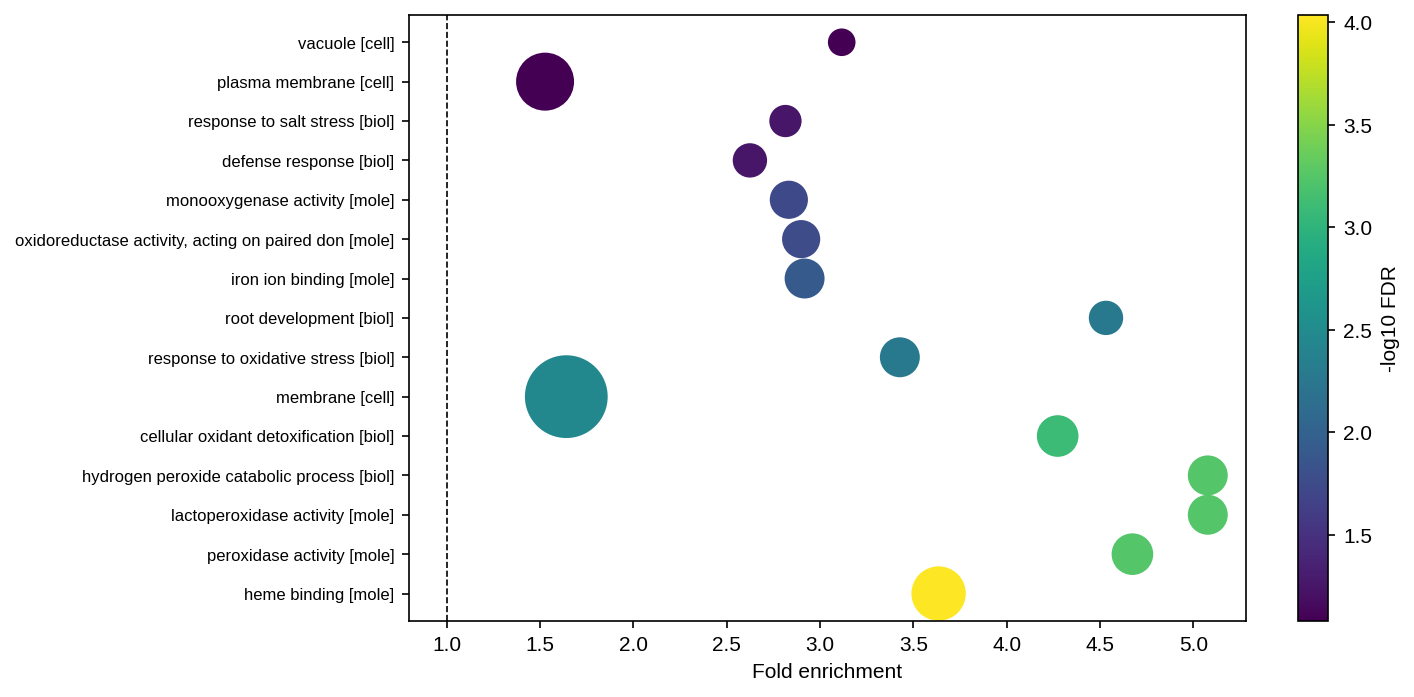
\includegraphics[width=\linewidth]{fig23_go_dotplot.png}\caption{}\end{subfigure}
\begin{subfigure}{0.49\textwidth}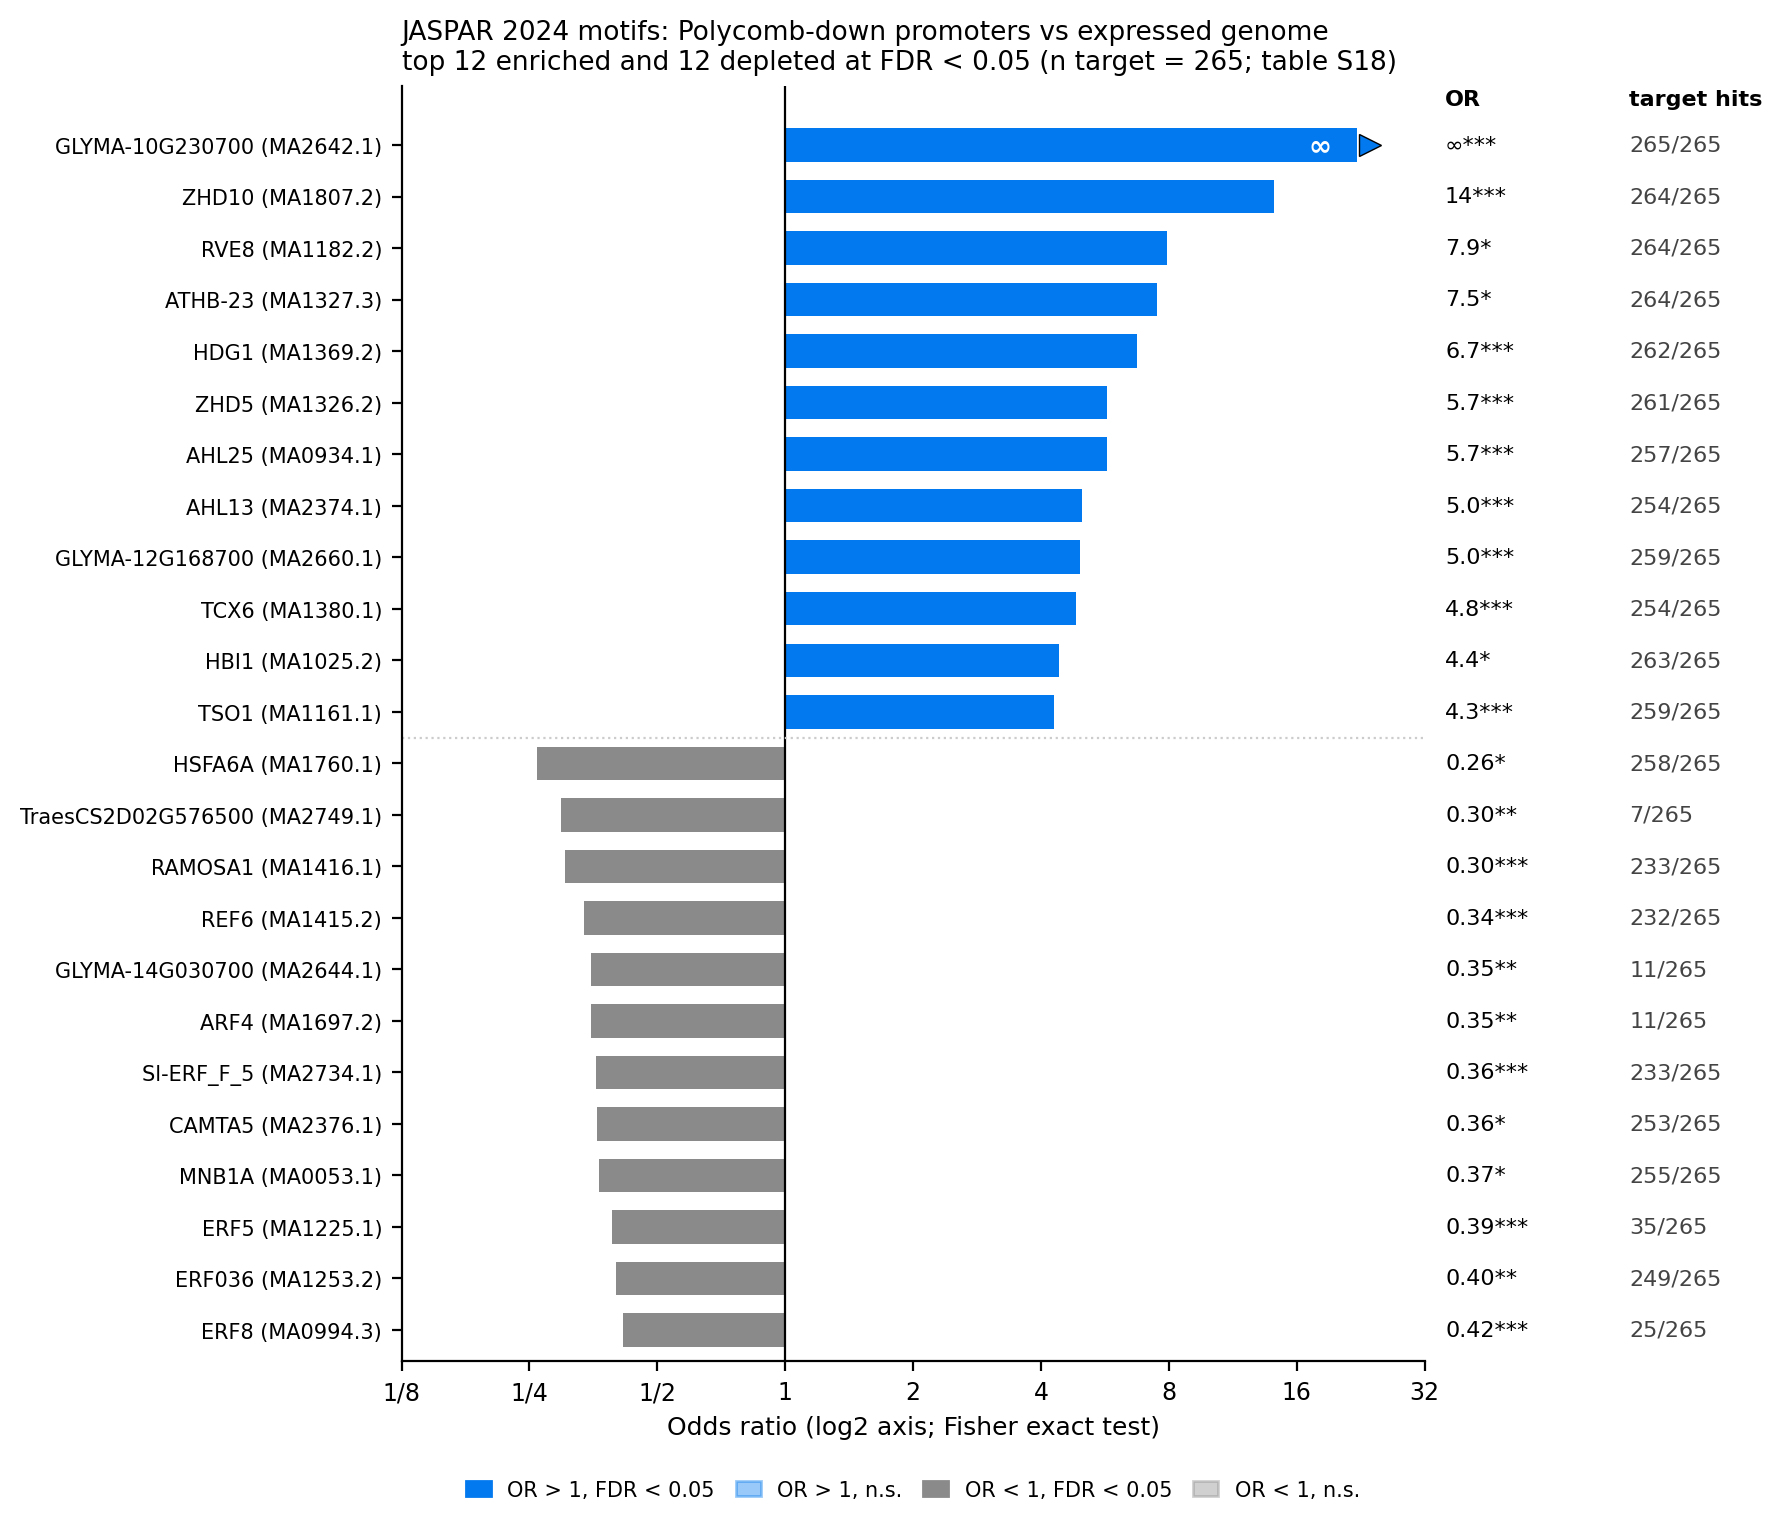
\includegraphics[width=\linewidth]{fig22_motif_enrichment.png}\caption{}\end{subfigure}\\[4pt]
\begin{subfigure}{0.6\textwidth}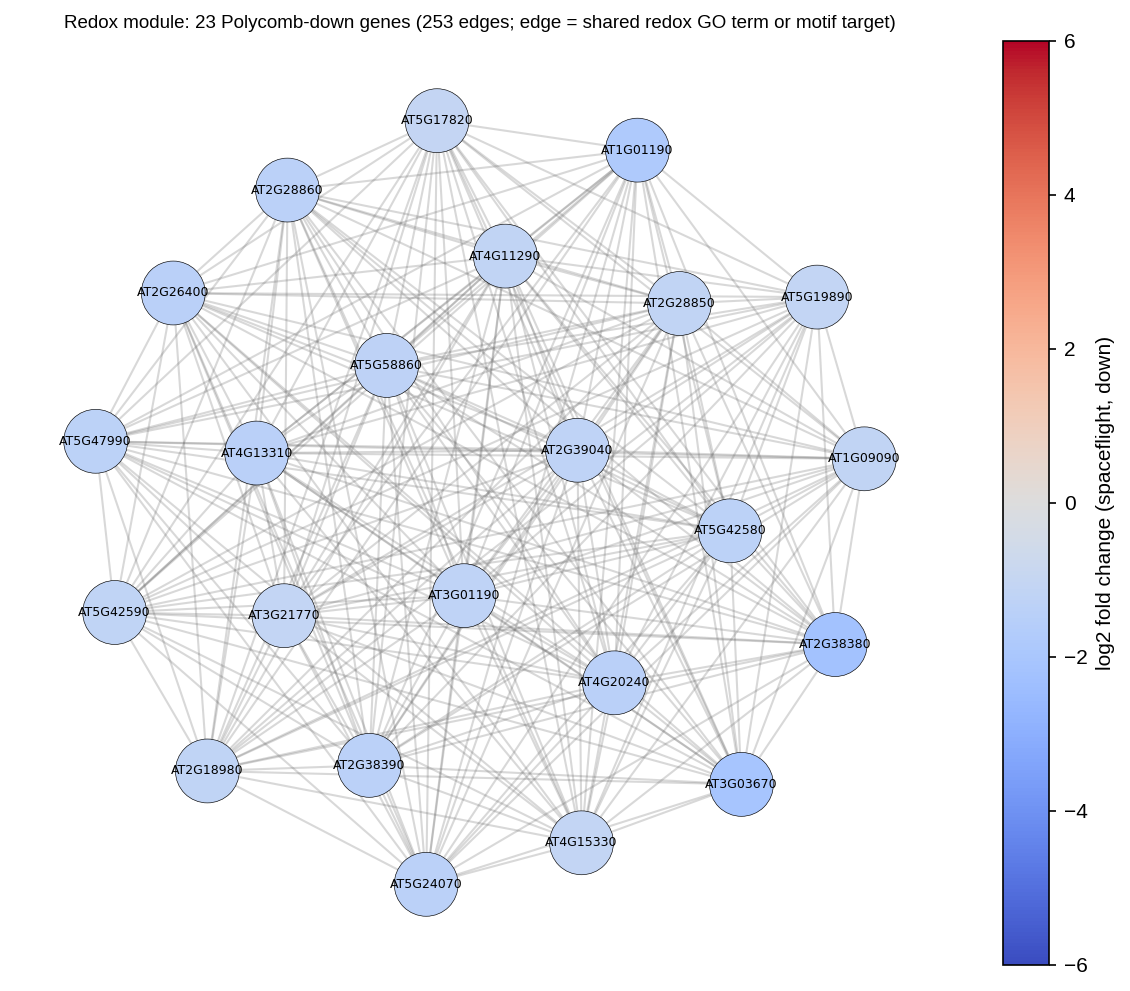
\includegraphics[width=\linewidth]{fig27_redox_network.png}\caption{}\end{subfigure}
\caption{\textbf{The repressed Polycomb class is a redox/peroxidase module.} (a) GO
over-representation against the genome and against the state-matched Polycomb control
(\Sx{19}). (b) JASPAR motif odds ratios in Polycomb-down promoters (\Sx{18}). (c) The
23-gene redox module, connected by shared redox GO terms or shared top-motif targets.
Node colour is the spaceflight log$_2$FC (Table~D3).}
\label{fig:module}
\end{figure}

\begin{figure}[p]
\centering
\begin{subfigure}{0.52\textwidth}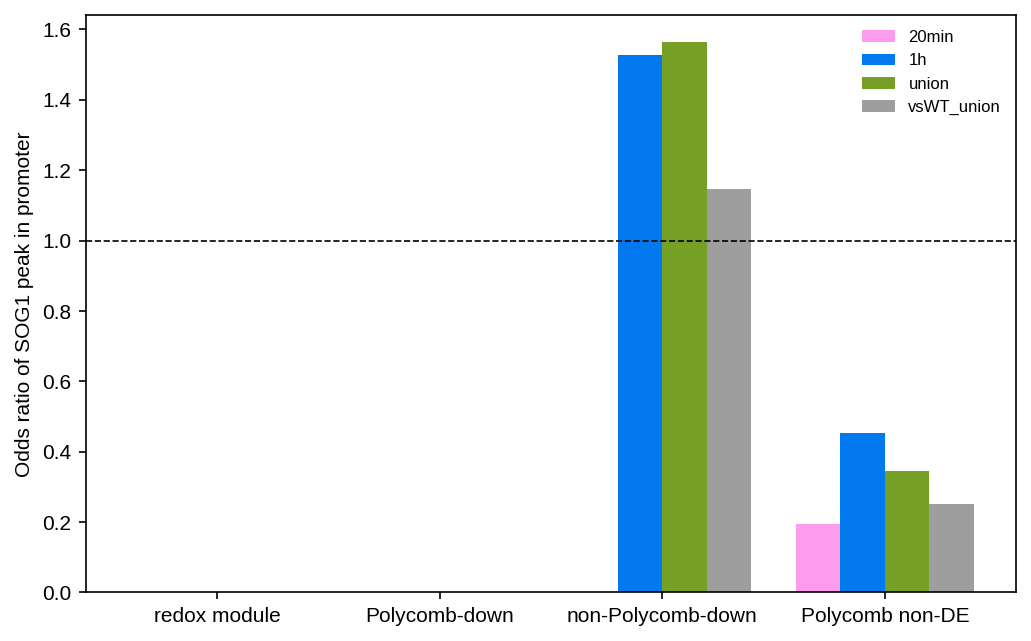
\includegraphics[width=\linewidth]{fig33_sog1_enrichment.png}\caption{}\end{subfigure}
\begin{subfigure}{0.46\textwidth}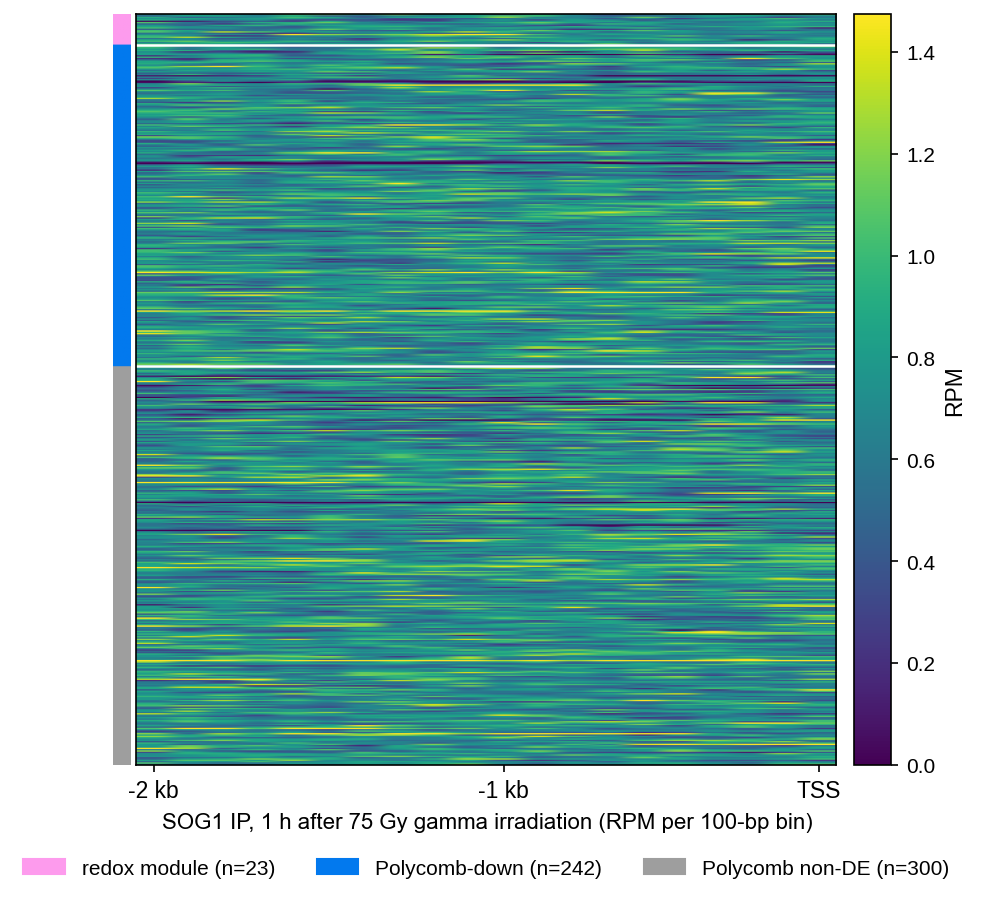
\includegraphics[width=\linewidth]{fig34_sog1_occupancy.png}\caption{}\end{subfigure}
\caption{\textbf{SOG1 does not bind redox-module or Polycomb-down promoters after DNA
damage (OSD-496).} (a) Fraction of promoters with a SOG1 peak, per gene set and timepoint
(\Sx{26}). (b) 1-h SOG1 promoter occupancy (RPM per 100-bp bin) by gene set.}
\label{fig:sog1}
\end{figure}

\begin{figure}[p]
\centering
\begin{subfigure}{0.62\textwidth}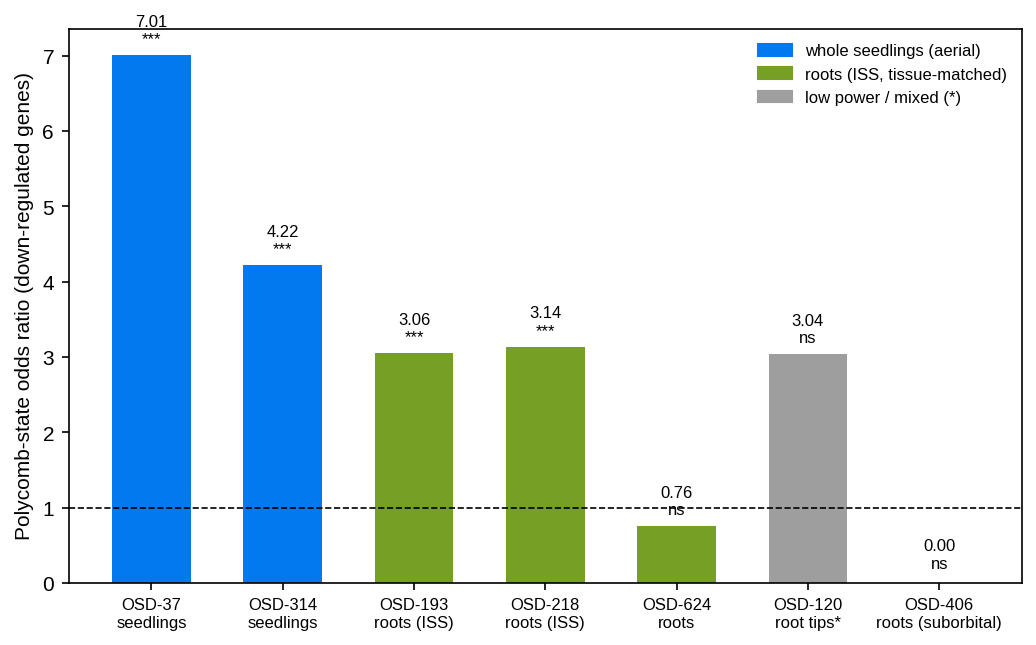
\includegraphics[width=\linewidth]{fig35_root_replication.png}\caption{}\end{subfigure}\\[4pt]
\begin{subfigure}{\textwidth}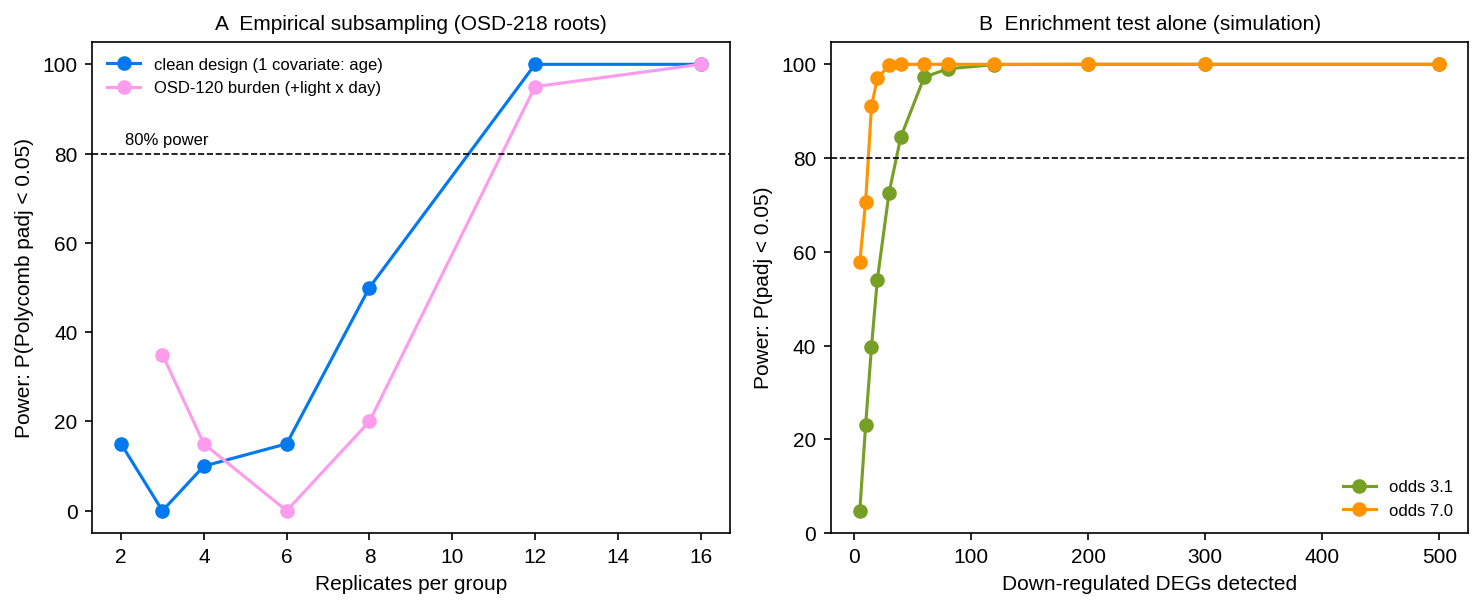
\includegraphics[width=\linewidth]{fig36_power_analysis.png}\caption{}\end{subfigure}\\[4pt]
\begin{subfigure}{\textwidth}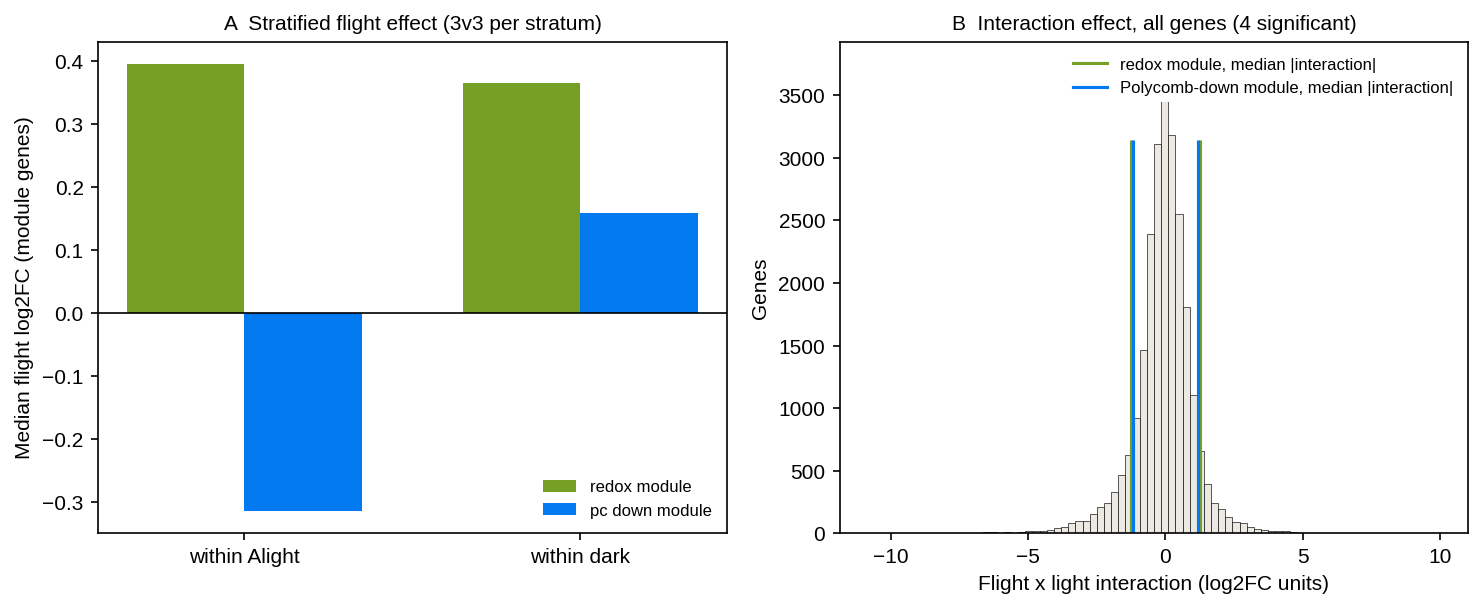
\includegraphics[width=\linewidth]{fig37_stratified_interaction.png}\caption{}\end{subfigure}
\caption{\textbf{Root replication, power and the OSD-120 interaction bound.}
(a) Polycomb-state odds ratio of down-regulated genes per dataset, as computed in v8 (Tables~S29, S32,
S34, S37, S39, S41). The OSD-314, OSD-218 and OSD-406 bars use the v8 contrasts; Fig.~\ref{fig:qc} gives their
corrected values. OSD-624 and OSD-406 are suborbital flights. (b) Power by replicates per group (empirical OSD-218 subsampling) and
by number of down-regulated DEGs (simulation; Tables~S42--S43). (c) OSD-120 Col-0 WT
flight effect within each light stratum and the gene-level condition $\times$ light interaction
(Tables~S44--S47).}
\label{fig:roots}
\end{figure}

\begin{figure}[p]
\centering
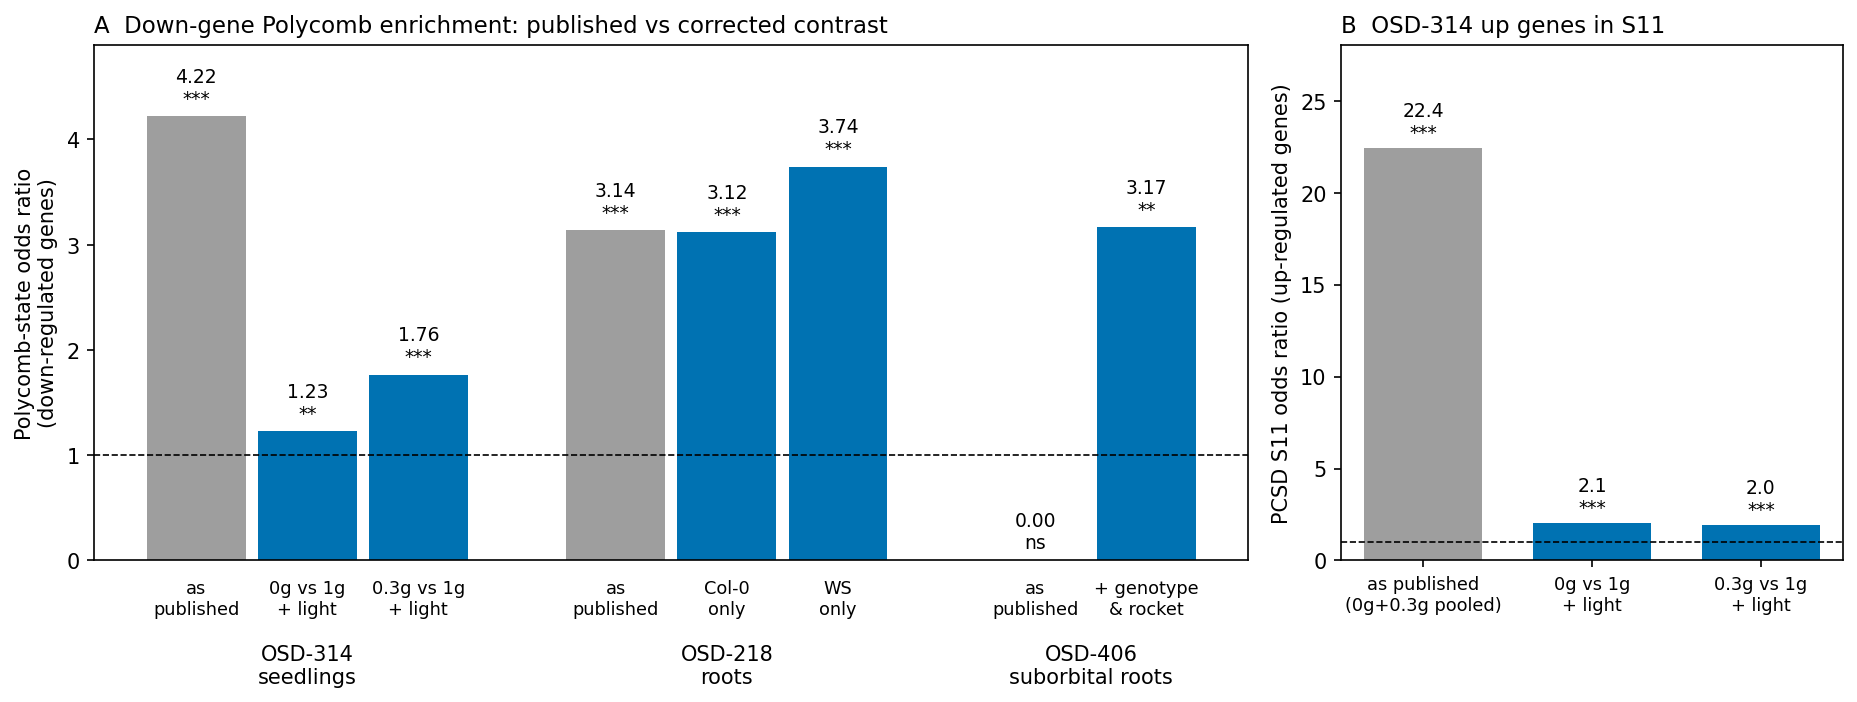
\includegraphics[width=\textwidth]{fig38_qc_corrections.png}
\caption{\textbf{What the pre-submission audit changed.} (a) Down-regulated-gene Polycomb (5-group) odds ratio
under the published contrast (grey) and the corrected contrast (blue). OSD-314: the published contrast pooled 0\,g
and Mars 0.3\,g against 1\,g, and the corrected contrasts separate the arms and add light as a covariate (\Sx{54}).
OSD-218: the published run pooled Col-0 and WS, and the corrected runs split them by genotype (\Sx{48}). OSD-406: the
published run pooled three genotypes and two rockets without covariates (\Sx{48}). (b) OSD-314 up-regulated genes in
PCSD state S11, published vs corrected. Stars: BH-FDR $<0.05$ (*), $<0.01$ (**), $<0.001$ (***). Generated by
\texttt{code/qc\_figure.py}.}
\label{fig:qc}
\end{figure}

% =====================================================================
\section{Discussion}

Three findings organise this work. First, \textbf{spaceflight repression is
chromatin-state-biased}. Down-regulated genes concentrate in Polycomb-repressed,
promoter-accessible euchromatin across datasets, tissues and state resolutions, while
constitutive heterochromatin is inert. The bias is not expression-driven, since the learned layer
fails honestly, and it is not explained by promoter GC content (state-matched controls).

Second, \textbf{the repressed class is a coherent redox/peroxidase module}. It is
distinguishable within the Polycomb class by function (11 GO terms) but not by promoter
motif architecture: the AHL/ZHD motifs track the state, not the response. This decouples
``which genes are in Polycomb states'' from ``which Polycomb genes respond to
spaceflight'', which is the central question the project reduces to.

Third, \textbf{the mechanism is not the canonical damage pathway}. SOG1, the
strongest candidate Polycomb-recruiting TF with available ChIP-seq, does not bind the
module's promoters after DNA damage. Together with the methylation nulls, this leaves the driver of the
state bias unidentified. Candidates include AHL/ZHD-family chromatin-associated
factors (the motif layer), light/circadian machinery, and campaign-specific hardware effects
(the OSD-624 null).

The power analysis turns the field's inconsistent root results into a design
requirement. Most root datasets in OSDR are underpowered for this test by a factor of two
or more, and a stratified reanalysis cannot rescue an underpowered factorial design.
The practical upshot is that the Polycomb-state bias is a robust, replicable feature of the
\textit{Arabidopsis} spaceflight transcriptome. The field needs a spaceflight
H3K27me3 ChIP-seq or CUT\&RUN assay with $\ge$10 replicates per group to convert the
ground-state-decoded bias into a demonstrated dynamic mark change.

\subsection*{Limitations}

\begin{itemize}
\item All chromatin states are \textbf{ground-state annotations}. The decoder tests
  enrichment of response genes in pre-existing states, not dynamic mark changes.
\item OSD-193 and OSD-218 share a payload and lab. OSD-624's null may reflect DE depth (36 down
  genes) or genuine campaign differences, and tissue is confounded with campaign.
\item Motif and GO findings are correlative and discovery-only; AHL/ZHD binding has not been validated by
  DAP-seq or ChIP.
\item Methylation tests are power-limited (3 replicates; 14--72 module genes in Ws) and
  ecotype-mismatched to the Col-0 discovery datasets.
\item The SOG1 ChIP-seq is from bleomycin-treated, mixed Ler/Col seedlings at two timepoints.
  Binding under other damage regimes or in other tissues is not excluded.
\item The power curve inherits OSD-218's effect size and dispersion, and the OSD-120
  stratified strata (3 v 3) are $\sim$0--15\% powered, so the interaction result is a bound.
\item OSD-406 and OSD-624 are suborbital (minutes of microgravity), and the EMCS partial-gravity datasets
  cannot answer the FLT/GC question as designed.
\item The OSD-314 diagnostics, GO replication and gene list (Tables~S13--S17, S21) describe the published pooled
  0\,g + 0.3\,g contrast. The corrected contrasts (Table~S54) show the same direction at a much smaller magnitude,
  and the 0\,g arm may be batch-confounded.
\end{itemize}

% =====================================================================
\section{Methods}

\subsection*{Pipeline}
Python 3.11. The core module \texttt{chromdecode.py} provides: ID harmonisation
(\texttt{clean\_agi}); counts loading; DE (\texttt{differential\_expression\_any}: linear models
on $\log_2$(counts) with condition + covariates, BH-FDR); coordinate mapping (TAIR10
\citep{berardini2015tair}, TSS-anchored gene body + 2\,kb); state assignment (PCSD 36-state segments,
AraENCODE 12-state seedling track, in which 8 of the 12 state labels occur at gene TSSs; PlantCADB ACR overlap); enrichment (Fisher exact, BH-FDR); and an
expression-only fallback decoder. A check script (\texttt{test\_chromdecode.py}) runs 21
checks on loci with known annotations.

\subsection*{Data}
PCSD (36 ChromHMM states, 290,553 segments) \citep{liu2018pcsd}; AraENCODE (12 states,
TPM matrix, gene annotation) \citep{wang2023araencode}; PlantCADB ACRs \citep{ding2023plantcadb}; NASA OSDR
metadata API and GeneLab-processed counts \citep{gebre2025osdr,berrios2021genelab}; JASPAR 2024 plant PFMs
\citep{rauluseviciute2024jaspar}; TAIR GO annotations and \texttt{go.obo} \citep{go2023knowledgebase}; and the TAIR10 genome. The source
data are not redistributed. Accessions and expected paths are listed in
\texttt{DATA\_SOURCES.md}.

\subsection*{ChIP-seq reanalysis}
HISAT2 2.2.1 on an index built from TAIR10 (single-end, \texttt{--no-spliced-alignment}); samtools
sort/index; MACS2 2.2.9.1 \texttt{callpeak} (\texttt{-f BAM -g 1.2e8 -q 0.01}; IP vs
matched-timepoint input; wild-type-IP specificity check). Promoter overlap uses strand-aware 2\,kb TSS
intervals, tested with Fisher's exact test against an expressed non-DE background and BH-FDR. Occupancy is
samtools per-100-bp bin counts scaled to RPM. The commands are in \texttt{code/hpc/sog1\_alignment.md}.

\subsection*{Metadata forensics}
NCBI E-utilities (esearch + esummary, db=biosample) for GSM/SAMN sample IDs; titles were parsed
into condition, age, genotype and replicate. Median-ratio size-factor scaling was used where
only unnormalised counts exist.

\subsection*{Power and interaction analyses}
Empirical power: the full pipeline was re-run on $k\in\{2,3,4,6,8,12,16\}$ replicates per group subsampled
from OSD-218, with 20 draws per $k$, with and without two random binary nuisance covariates
mimicking OSD-120's light $\times$ day design. Analytic power: simulated Fisher tests at
odds 3.1 and 7.0 against a background fraction of 0.141. Interaction: gene-wise linear model
expression $\sim$ condition + light + condition:light on the 12 OSD-120 Col-0 WT samples,
with BH-FDR across genes.

\subsection*{Pre-submission audit and corrections}
Before submission, every dataset's platform, genotypes and design were re-read from its OSDR study record and
NCBI BioSample titles. Every sweep result was then regenerated from the public counts with the pinned
environment (\texttt{code/qc\_sweep\_rerun.py}, \texttt{code/qc\_genotype\_rerun.py}). The re-run reproduced the
archived counts and odds ratios exactly (\Sx{50}; S48, first two rows), and it found four problems, all
corrected in the text above.
(i) OSD-314's Mars-gravity samples (``03g'') were not parsed, and the contrast coding counted them as
treatment (Table~S53).
(ii) The BioSample parser did not recognise ``WS'', so OSD-218's 16 WS samples entered a contrast described as
Col-0.
(iii) OSD-406 was described as Col-0, but it holds Col-0, WS and \textit{sku5} from two rockets.
(iv) OSD-624 was described as an orbital dataset; it is a Virgin Galactic suborbital flight.
Two archive-level problems were also fixed. The 5-group sweep table exported from the analysis workspace
predated the log$_2$ correction, and it has been replaced by a regenerated table (\Sx{51}). The significance stars
in the original 5-group heatmap were misaligned by a column-order bug in \texttt{aggregate\_sweep.py}.
Downstream analyses built on the original OSD-314 and OSD-218 gene sets (the OSD-314 diagnostics and GO
replication, the power subsampling, and the OSD-120 module bound) were not re-run, and are labelled as such where
they are reported.

\subsection*{Statistics}
Fisher exact (one-sided where enrichment is directional); BH-FDR within test families;
hypergeometric GO over-representation; permutation-based null calibration and GSEA
(1,000--10,000 draws); genomic-block CV for the learned layer. Thresholds are padj $<0.05$
and $|\log_2\mathrm{FC}|>1$ unless stated. All results are discovery-only.

% =====================================================================
\section*{Data availability}
All result tables are in \texttt{supplementary\_tables/} (Tables S1--S57, indexed in its
\texttt{README.md}), with small derived data in \texttt{data/derived/} (Tables D1--D7). All
50 figures (SVG + PNG) are in \texttt{figures/}. The complete per-version project record is
\texttt{reports/report\_chromdecode\_at.md}. Source data are public and listed in
\texttt{DATA\_SOURCES.md}. Repository: \url{https://github.com/dr-richard-barker/ChromDecode-At}.
Archived release: Zenodo DOI to be assigned on first release.

\section*{Code availability}
All 29 analysis scripts are in \texttt{code/} (MIT licence). \texttt{chromdecode.py} is the
core module.

\section*{Competing interests}
The author declares no competing interests.

\bibliographystyle{unsrtnat}
\bibliography{references}

\end{document}
